%The fwahl LaTeX template made for use at Uni Passau

\documentclass[12pt, a4paper, onecolumn, oneside, parskip=half]{scrartcl}

\title{Machine Learning Project Report}

%%%%%%%SETUP BEGIN%%%%%%%
%Define constant names, etc.
\newcommand{\authors}{Maryam Nouhnejad, Haythem Sahbani, Jakob Wasserthal
} %List Authors here
\newcommand{\prof}{Prof. Dr. Amft, Dr. Reiss} %List Prof here
\newcommand{\doctitle}{Machine Learning and Context Recognition Project Report} %Document Title
\newcommand{\subcode}{code} %Subject Code
\newcommand{\docsubject}{Intensity estimation: classification vs. regression} %Subject name, also appears in header
%\newcommand{\centerhead}{Assignment Y} %Center part of header
\newcommand{\centerfoot}{University of Passau} %Center part of footer
%%%%%%%SETUP END%%%%%%%%

\usepackage{graphicx}
\usepackage{a4wide}
\usepackage{color}
\usepackage{listings}
\usepackage{float}
\usepackage{amsmath}
\usepackage{mathtools}
\usepackage{booktabs}
\usepackage{footmisc}
\usepackage{sectsty}
\usepackage[headsepline,footsepline]{scrpage2}
\usepackage{hyperref}
\usepackage{titlesec}
\usepackage[colorinlistoftodos]{todonotes}
\usepackage{wrapfig}
\usepackage{float}

\newcommand{\fwa}[1]{\todo[author=Florian, color=blue!40,  inline]{#1}}
\newcommand{\oam}[1]{\todo[author=Oliver, color=red!40,  inline]{#1}}

% Nonindented footnotes
\setlength{\footnotemargin}{2mm}

% Prevent PDF Version warnings
\pdfminorversion=6

% Colors
\definecolor{darkblue}{rgb}{0.0,0.0,1}
\definecolor{midgreen}{rgb}{0.0,0.5,0.0}
\definecolor{lightgray}{gray}{0.95}

% Listings
\lstset
{
	language=Matlab,
	frame=single,
	backgroundcolor=\color{lightgray},
	showstringspaces=false,
	keywordstyle=\bfseries\color{darkblue},
	commentstyle=\color{midgreen},
	basicstyle=\ttfamily\fontsize{8}{8}\selectfont,
	numbers=left,
	captionpos=b,
	breaklines=true,
	aboveskip=\baselineskip,
	tabsize=2
}

% New commands
\newcommand{\HRule}[2]{\noindent\rule[#1]{\linewidth}{#2}}
\newcommand{\vlinespace}[1]{\vspace*{#1\baselineskip}}

% TOC
\setcounter{tocdepth}{2}

% PDF attributes and link colors
\hypersetup
{
  pdftitle={\doctitle{}},
  pdfauthor={\authors{}},
  pdfsubject={\subject{}},
	colorlinks=true,
  linkcolor=black,
  citecolor=black,
  filecolor=black,
  menucolor=black,
  urlcolor=black
}

% Header and footer
\ihead{\docsubject{}}
\chead{\




{}}
\ohead{\today}
\ifoot{\headmark}
\cfoot{\centerfoot{}}
\ofoot{\thepage}
\automark[section]{section}

% Redefine headings
\titleformat{\section}{\sffamily\LARGE\bfseries}{\thesection}{1em}{}
\titleformat{\subsection}{\sffamily\Large\bfseries}{\thesubsection}{1em}{}
\titleformat{\subsubsection}{\sffamily\large\bfseries}{\thesubsubsection}{1em}{}
\titleformat{\paragraph}{\sffamily\normalsize\bfseries}{\theparagraph}{1em}{}
\titleformat{\subparagraph}{\sffamily\small\bfseries}{\thesubparagraph}{1em}{}

\begin{document}

\begin{titlepage}

\sffamily

\includegraphics[width=5cm]{pictures/actlabLogo.png}
\hfill \centering

\includegraphics[width=7cm]{pictures/uplogo.png}
\HRule{10pt}{2pt}

\vfill
\Large{\docsubject{} \\\subcode{} \\}
\vlinespace{1}
\huge{\doctitle{}\\}
\vlinespace{10}
\vfill
\large
by \authors{}\\
\vfill
%\vlinespace{5}
\HRule{10pt}{2pt}
\raggedright
\textbf{Date: } \today{} \\
\textbf{Professor:} \prof{}

\end{titlepage}
\pagenumbering{Alph}

%Abstract here
%\section*{Abstract}
%newpage %adds page break between Abstract and TOC
\tableofcontents
\newpage
\pagestyle{scrheadings}
\pagenumbering{arabic}



%Text goes here
\section{Introduction}
Trends like "quantify yourself" are becoming more and more prominent these days. Given the rising awareness for health and fitness for a broad spectrum of society and given the ever increasing permeation of technology in society, those trends are obvious. For most of those fitness and quantify yourself applications, measurements of the environment and our body are necessary. This is done by the use of sensors that help to translate physical phenomenons into digital data which then can be processed by software. However, in the beginning the sensor outputs are only a huge amount of numbers. To make sense out of those numbers and to gain the information wanted, can be a challenging task. In the next section we will introduce the problem we are trying to solve in this domain.


\section{Intensity Estimation}

\subsection{Problem Statement}

In this project we focused on the problem of estimating the intensity levels of physical activities like sitting, running, vacuum cleaning, etc. by using different approaches of classification and regression and then compared the result to one another. What we tried to re-implement is important specially in health-care. Therefore by wearing sensors during activities, it would be possible to tell if someone is performing enough physical activity to maintain or promote his health. The type, duration, and intensity of the activities are all important, but in this project, we only focused on estimating the intensity level.

The intensity levels are defined by Metabolic Equivalent of Task (MET), which is explained in \cite{met_paper}. MET is the ratio of work metabolic rate to a standard resting metabolic rate of $1.0 (4.184  kJ)\cdot kg^{-1}\cdot h^{-1}$. It is a measure that expresses the energy cost of a physical activity and is defined as the ratio of metabolic rate (and therefore the rate of energy consumption) during a specific physical activity to a reference metabolic rate. 1 MET is equal to a resting metabolic rate obtained during quiet sitting. Each activity has a metabolic equivalent intensity level that ranges from 0.9 (sleeping) to 18 (running at 10.9 mph). 

\begin{figure}[ht!]
  \centering
  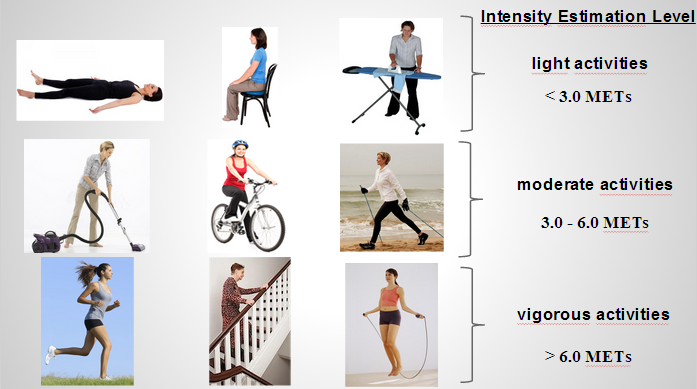
\includegraphics[width=160mm]{pictures/nine_activities.png}
  \caption{Intensity Estimation Levels
  \label{intensity_levels}}
\end{figure}

Three classes of intensity are defined to distinguish various physical activity tasks in this problem: light, moderate and vigorous (according to the work in \cite{Attila_2012}); and they are distinguished using MET values, as such: light activities have a MET value less than 3, moderate activities between 3 and 6, and vigorous activities have a MET value more than 6; this is depicted in the figure \ref{intensity_levels}. The result of this computation would be sufficient for general health applications, e.g. (as has been explained in \cite{ACSM}) to observe and check if physical activity done by a person is enough to be counted towards daily physical activity and if a combination of moderate and vigorous intensity physical activity was performed. Therefore rather than focusing on predicting MET values in this study, we used them as a threshold to estimate the type of intensity level.


\subsection{The Dataset}

We used a physical activity monitoring dataset, called PAMAP2 \cite{PAMAP_2}. Three inertial measurement units (IMU) and a heart rate monitor with a sampling frequency of 100 Hz and 9 Hz respectively, were used as sensors during the data collection to record the heart rate and acceleration data.
The sensors were lightweight and small, and they were positioned over the wrist on dominant arm, on the chest, and one the dominant side's ankle.

Nine subjects participated in the data collection phase, and they were mainly employees or students, one female and eight males, aged $27.22\pm3.31$. Each of the subjects had to follow a protocol, containing 12 different activities, performing each in the way most suitable for himself. The protocol is shown in table \ref{protocol_12_activities}.

\begin{table}ht!]
  \centering
  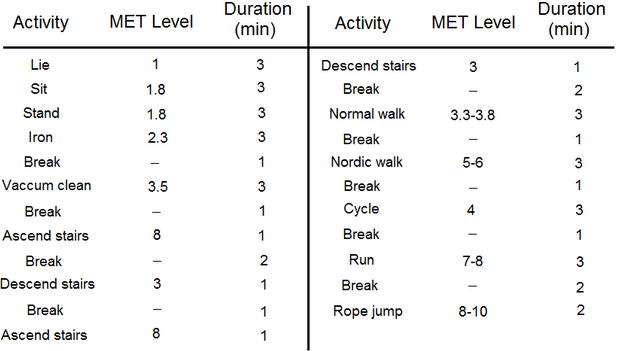
\includegraphics[width=155mm]
  {pictures/protocol.png}
  \caption{The Protocol \label{protocol_12_activities}}
\end{table}

Most of the activities during the data collection protocol were performed over approximately 3 minutes, except ascending/descending stairs (due to the limitations of the building where the indoor activities were carried out) and rope jumping (to avoid exhaustion of the subjects). The activity lying refers to lying quietly while doing nothing.

Break intervals are added between the activities of the protocol, so that the heart rate of the subjects returns into the normal range after performing an activity; in another word, the measured heart rate values within the activity wouldn't be affected by the previously performed activities. For vigorous and exhausting activities such as ascending stairs and running, a 2-min break is enough, but for others, only 2-min break was inserted. However, some of these breaks were deleted, since in real life, different activities may happen after one another, so that the influence of each on the next performed ones cannot be excluded, this influence was also simulated in the data collection protocol with descending stairs directly after ascending stairs.

A text file was available for every subject, containing synchronized and labeled raw data from all the sensors. Since the IMUs had a sampling frequency of 100 Hz, data was sent every 0.01 second and if any data such as HR-values was missing due to wireless data dropping, they were indicated with NaN in the data-files.

Second column of the data set was activityID (i.e. 3 for standing, 6 for cycling). Data labeled with activityID equal to zero were discarded in the analysis, because it indicated transient activities between performing different activities, e.g. going from one location to the next activity's location.

The ground truth for the activity recognition task is provided by the labels made during data collection. In addition, a period of 10 seconds from the beginning and end of each performed activity were discarded to avoid transient data. To obtain reference data, it is sufficient to only use the compendium of physical activities, because our task is to estimate the intensity levels, not the exact MET values.



\section{Data Processing }

Raw data is generally not well fitted for the needs of a project.  This can be driven by the lack of attribute values or certain attributes of interest. Also real world data is noisy. It contains errors or outliers.  Therefore the data needs to be processed. At this end, we processed the data as shown in figure (\ref{fig:classifier-pipeline}):

\begin{figure}[H]
  \centering
  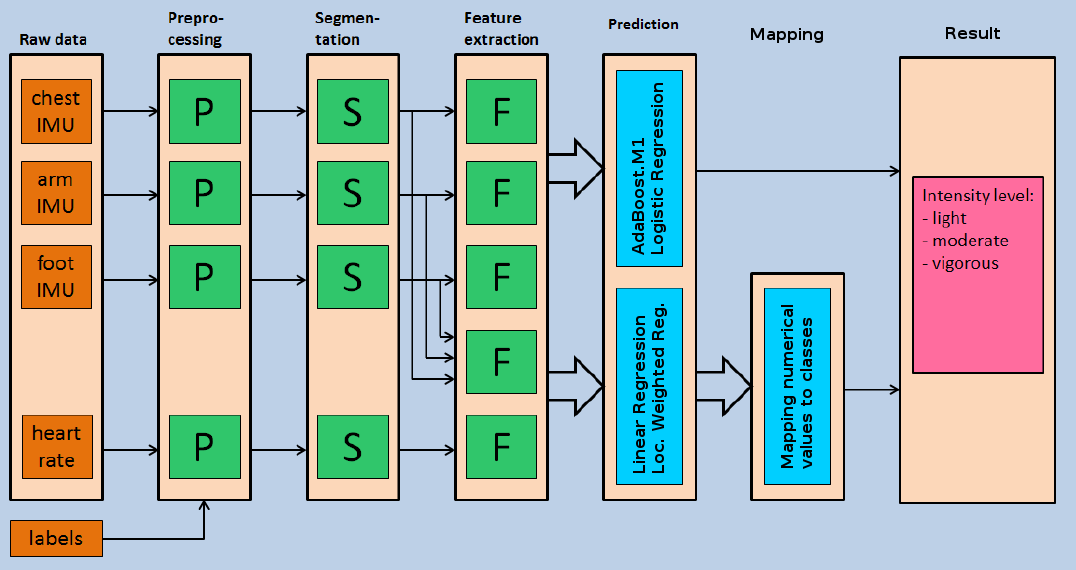
\includegraphics[width=160mm]{pictures/Data_process_chain.png}
  \caption{Data processing chain \label{fig:classifier-pipeline}}
\end{figure}

 
The dataset we worked on has already been preprocessed and labeled. Therefore this step is already done. In the next sections we will discuss how we segmented the data and which features we used to get best results for the different algorithms. 
From the sensor input we only used the heart rate and the acceleration IMU data. The temperature, gyroscope data and magnetometer data do not give a lot of indication for the kind of activity.

\subsection{Segmentation}
As mentioned before, the goal of the project is to classify activities into three levels of intensity. In this part, we should classify static activities. Therefore we proceeded to the data segmentation as follow:

At first, we removed the breaks from the data points, since that kind of information is not relevant for the classification task.

In the next step, we took only the static phase of an activity. Since each activity period is between 1 to 3 minutes, we deleted the first and last 10 seconds of each activity. We assumed that deleting more would result in reducing the number of data points for the classification algorithm and so we would diminish the accuracy of the classifier.

After that, we segmented the data into windows of 5.12 sec length each. We supposed that in this time period, the activity is in a constant level of intensity and thus the data contained in this window is relevant for the actual intensity level of the activity.

The whole process is shown in figure \ref{Activity segmentation process}.

\begin{figure}[H]
  \centering
  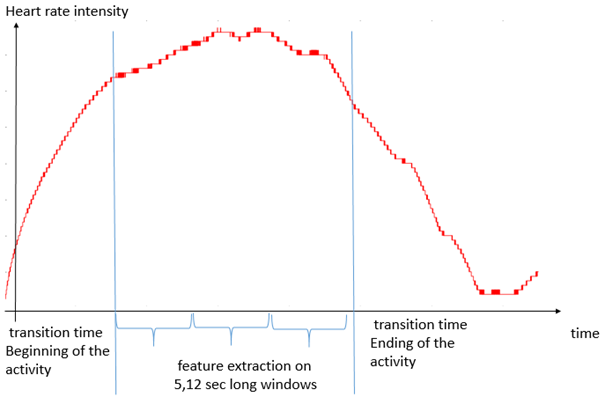
\includegraphics[width=160mm]{pictures/Data_segmentation.png}
  \caption{Activity segmentation process \label{Activity segmentation process}}
\end{figure}



In the upcoming section we will discuss the next step of data processing, which is feature extraction.

\subsection{Feature Extraction}

The final section for processing the data is feature extraction. This part is influenced by the machine learning algorithms that will be used to classify the activities in the next step. In this way, feature engineering is really important and it strongly affects the final results. Also, we revisited this part as we progressed in the project work.

\textbf{Heart rate feature extraction}

The heart rate data points are naturally relevant for an activity level classification. Nevertheless the metabolism is different for each subject. The subjects are different in gender, age and even in their daily life activities. For example, the heart rate would not be the same for a student who practices sports and another one who prefers playing video games. To remedy to this natural fact, the heart rate has been normalized independently for each subject using equation (\ref{eq:heart_rate_normalization}):
 
\begin{equation}
\label{eq:heart_rate_normalization}
normalized_{hr} \leftarrow \frac{max_{hr} - hr}{max_{hr} - min_{hr}}
\end{equation}

Where: 
$$max_{hr}   \text{ is the maximum heart rate of a subject}  $$ 
$$min_{hr}   \text{ is the minimum heart rate of a subject}  $$


\textbf{Acceleration IMU feature extraction}

The acceleration IMU observations are far too voluminous in their raw state to be modeled by predictive modeling algorithms directly. After looking into different scientific papers that are related to this subject we found that the features extracted from this kind of data are peak acceleration, mean, median, standard deviation absolute integral  \cite{Attila_2012}\cite{Attila_2013}.
Extracting all these features seems pointless because it does not add a lot of information for the classifier. Also it would increase computation time and memory consumption. Thus we decided to extract these two features:
\begin{itemize}
\item Standard deviation: used a numpy built-in function for computation
\item Energy: the sum of the squared discrete FFT component magnitudes of the signal. The sum was divided by the window length for normalization. 
\end{itemize}

Choosing these features has the following goals:
\begin{itemize}
\item Pairing frequency and time domains gives better accuracy for the classifier.
\item Standard deviation is a good variation measurement.
\item Energy is a power measurement.
\end{itemize}



After extracting the features, it came to our attention that the preprocessed data contains attributes with a mixture of energy and standard deviation scale. It is a good point to rescale these features. Also another feature engineering method that improves the accuracy of the classifier is feature standardization. This method puts the mean to zero and the standard deviation to 1 for each feature.

%\textbf{Result of data preprocessing}

%In the figure (\ref{fig:Data preprocessing result}) we can see that there are much less data points. This is a result of segmentation and feature extraction.

%\begin{figure}[H]
%  \centering
%  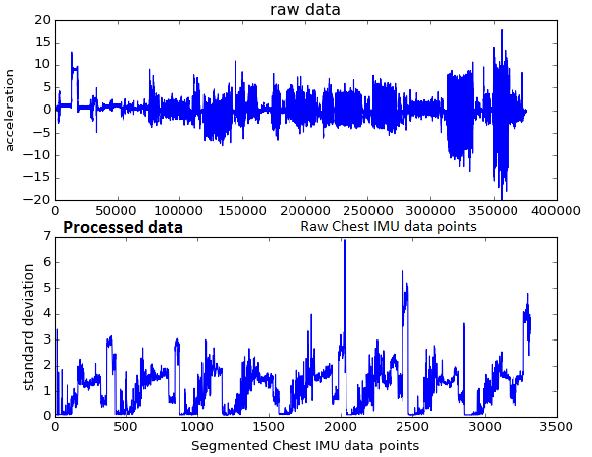
\includegraphics[width=130mm]{pictures/feature_extraction.png}
%  \caption{Data preprocessing result\label{fig:Data preprocessing result}}
%\end{figure}

\subsection{Classification}

After extracting the features we can now come to the actual task of classification. A classifier takes a list of features as an input and then returns a prediction of what class this data point belongs to. Here we present two of these classifiers:
\begin{itemize}
\item AdaBoost.M1
\item Logistic Regression
\end{itemize}

Regression can also be used for classification. Regression is taking a list of features as an input and returns a numerical value, based on the function fitted on the training data. This numerical return value is not a class, so we have to introduce another step where we map those numerical values to actual classes.

This mapping is done in the following way: The labels for the regression algorithms are the MET values ranging from 0 to 9 in this dataset. For a new data point the regression is then predicting an MET value between 0 and 9. Now we simply map values between 0 and 3 to class "light", values between 3 and 6 to class "moderate" and values between 6 and 9 to class "vigorous". This way we can use regression for classification. Here we are also presenting two of these regression algorithms:
\begin{itemize}
\item Linear Regression
\item Locally Weighted Linear Regression
\end{itemize}


\section{Algorithms}

\subsection{Linear Regression}

Linear regression is an approach for modeling the relationship between a scalar variable “y” and one or more explanatory variables denoted “X”. The case of one explanatory variable is called simple linear regression. For more than one explanatory variable, the process is called multiple linear regression.\\
The linear regression tries to fit this equation: 

\begin{equation} 
 h_\theta(X)= y
\end{equation}


Figure \ref{Classifying heart rate using Linear least squares} is an example for fitting heart rate into activity level.\\
First, the heart rate point will be mapped to an MET value in a [0, 9] range. Then, this value will be compared to the threshold to get its intensity level.

\begin{figure}[H]
  \centering
  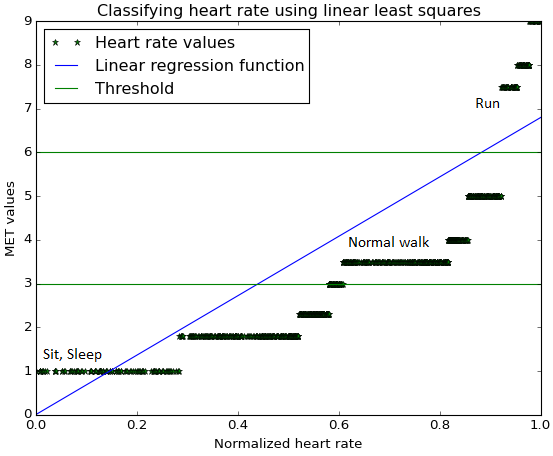
\includegraphics[width=130mm]{pictures/Linear_least_squares_plot.png}
 \caption{Classifying heart rate using Linear least squares} 
 \label{Classifying heart rate using Linear least squares}
\end{figure}

In the learning phase, the algorithm minimizes a cost function (\ref{eq:cost_function}) which is based on least squares approach. "Least squares" means that the overall solution minimizes the sum of the squares of the errors made in the results of every single equation. 

\begin{equation}
\label{eq:cost_function}
 J(\Theta)= \frac{1}{2m}\sum_{i=1}^{m}(h_\theta(\underline{x}^i)-y^i)^2
\end{equation}


%$$\Theta = (\theta_0, \theta_2, .., \theta_{n}), m is the number of features
%X = {matrix}
Where $$\Theta = \{\theta_0, \theta_1, \cdots, \theta_n\}\text{, n is the number of features used}$$
$$y = \{y^1, y^2, \cdots, y^m\}\text{, m is the number of data points}$$
\newcommand{\tab}[1]{\hspace{.2\textwidth}\rlap{#1}}
\tab{$ h_\theta(x^i) = \theta_0 + \theta_1\underline{x}_1^i + \cdots + \theta_n\underline{x}_n^i $ \text{, $\underline{x}^i$ is the feature vector }}




The cost function is minimized using the Gradient descent algorithm (\ref{eq:Gradient_descent_algorithm}):

% Start with initial parametres of \Theta = \theta_0, \cdots, \theta_n

Repeat until convergence \{

\begin{equation} 
\label{eq:Gradient_descent_algorithm}
\theta_j \leftarrow \theta_j - \alpha\frac{1}{m}\sum_{i=1}^{m}(h_\theta(\underline{x}^i)-y^i)x^i_j
\end{equation}
\}

(simultaneously update $\theta_{j} \ \text{for} \ j=0,1,...,n$)

Where $\alpha$ is the learning rate of the algorithm \cite{learning_rate}. Choosing the right value is crucial to gradient descent success. In fact, if the learning rate is too big, then gradient descent will diverge. For example  in figure \ref{fig:cost_function_plot}, we can see that if $\alpha$ is too large the cost function will go iteratively through these points: $(1 \rightarrow 3\rightarrow 7\rightarrow 4)$. The algorithm will miss the optimal solution which is point 8. In the other side, if $\alpha$ is too small gradient descent will be too slow for  converging .


\begin{figure}[H]
  \centering
  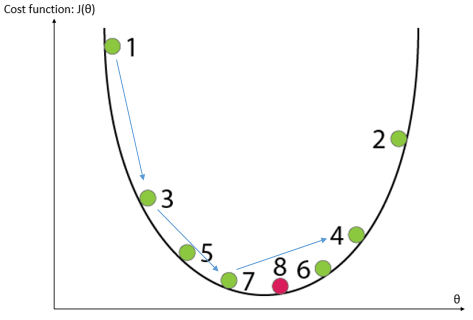
\includegraphics[width=130mm]{pictures/cost_function_of_theta_2.png}
  \caption{Plot of the cost function \label{fig:cost_function_plot}}
\end{figure}

The number of iterations of gradient decent is problem dependent. In figure \ref{fig:Minimizing the cost function} we see that after 300 iterations the cost function converges. We reached this result after testing multiple learning rate values. We finally took $(\alpha = 0.01)$ as the algorithms needs a descent number of iterations to learn from the different datasets.
At this point learning phase of the algorithm can be stopped. And we use the resulting $\Theta$ to predict the MET values.

\begin{figure}[H]
  \centering
  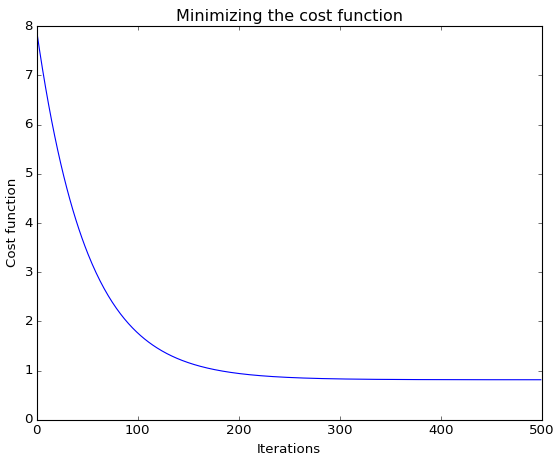
\includegraphics[width=130mm]{pictures/cost_function.png}
  \caption{Minimizing the cost function \label{fig:Minimizing the cost function}}
\end{figure}



\subsection{Logistic Regression}

Logistic regression is addressing binary classification. In contrast to linear regression, logistic regression is not trying to fit a linear function onto the data, but a sigmoid function. 

\begin{equation}
\label{eq:model_log_reg}
 h_\theta(X)= \frac{1}{1 + e^{-\theta^T x}}
\end{equation}

This results in the following cost function

\begin{equation}
\label{eq:cost_function_log_reg}
 J(\Theta)= -\frac{1}{m} \lbrack \sum_{i=1}^{m} y^{(i)} log(h_\theta(x^{(i)})) + (1-y^{(i)})log(1-h_\theta(x^{(i)})) \rbrack
\end{equation}

Where $$\Theta = \{\theta_0, \theta_1, \cdots, \theta_n\}\text{, n is the number of features used}$$
$$y = \{y^1, y^2, \cdots, y^m\}\text{, m is the number of data points}$$
%\newcommand{\tab}[1]{\hspace{.2\textwidth}\rlap{#1}}
\tab{$ h_\theta(x^i) = \theta_0 + \theta_1 x_1^i + \cdots + \theta_n x_n^i $ \text{, $x^i$ is the feature vector }}

Estimating the parameters of the sigmoid function is done with gradient ascent. This is a greedy iterative approach to find an optimum. A numerical solution does not always exist or is not always feasible to be computed. Gradient ascent offers a solution that also works in those cases where a closed form numerical solution is not possible.\newline

Repeat until convergence \{

\begin{equation} 
\label{eq:Gradient_descent_log_reg}
\theta_j \leftarrow \theta_j - \alpha\frac{1}{m}\sum_{i=1}^{m}(h_\theta(x^{(i)}) - y^{(i)}) x_j^{(i)}
\end{equation}
\}

(simultaneously update $\theta_{j} \ \text{for} \ j=0,1,...,n$)

The advantage of using a sigmoid function is that it gives back values between 0 and 1. Those can be interpreted as the probability that the input sample belongs to class 1 (see figure \ref{logistic_regression_concept}). 

\begin{figure}[ht!]
  \centering
  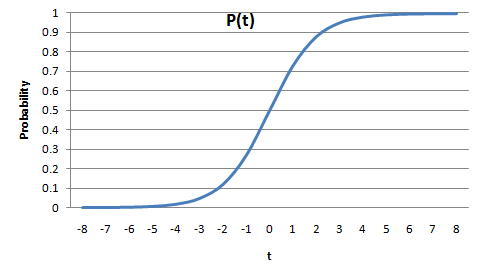
\includegraphics[width=110mm]{pictures/logistic_regression_concept.png}
  \caption{Logistic Regression Concept \label{logistic_regression_concept}}
\end{figure}

To do the actual classification we have to introduce a threshold. The threshold is simply 0.5. Any value above 0.5 means that the data belongs to class 1 and any value below 0.5 means that the data belongs to class 0.

The result of logistic regression for the heart rate data can be seen in figure \ref{logRegFitting}. The real values represent the measured heart rate for class "medium intensity" and class "low intensity". The predicted values show the values predicted by the sigmoid regression model. All the predicted values above the threshold line will be predicted as class "medium intensity", all the values below as "low intensity".

\begin{figure}[ht!]
  \centering
  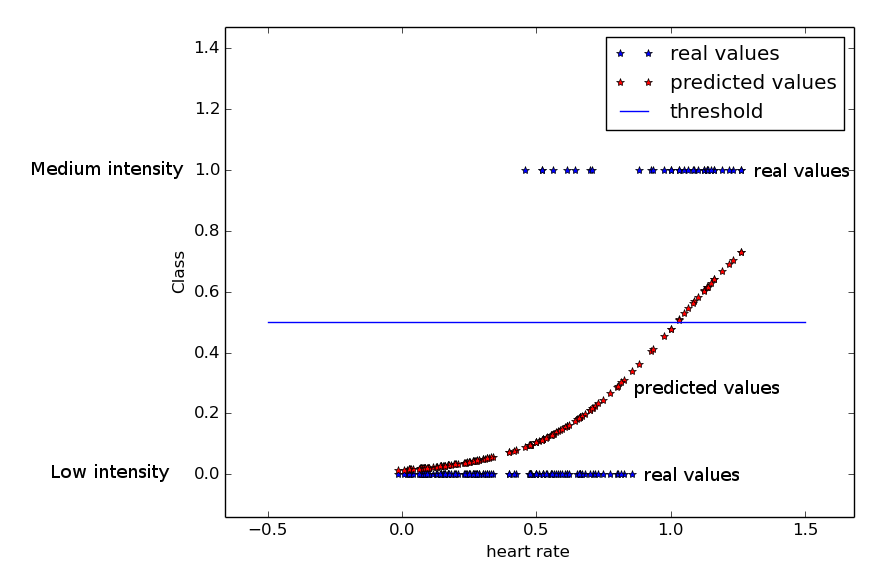
\includegraphics[width=110mm]{pictures/LogReg_fitting_1.png}
  \caption{Logistic Regression on heart rate feature \label{logRegFitting}}
\end{figure}

However, logistic regression is only for binary classification. As we are using three classes, we can not use it on its own. There are two ways how to use binary classifiers for multi-class classification:
\begin{itemize}
\item One-vs-all method \newline
For each class we train a logistic regression classifier which predicts the probability that a data point has this class. For a new data point we simply run all of these classifiers and then take the class which got the highest probability.
\item One-vs-one method\newline
In this method we take all pairwise combinations of the classes and for each one of them we train a logistic regression classifier. For a new sample we run all of these classifiers and the class  which was chosen by the most classifiers "wins" and is returned.
\end{itemize}
First we tried to use the One-vs-all method. This one is supposed to be less computational expensive as you do not have to train a classifier for each pairwise combination, but only for each class. Moreover the scikit learn implementation is using the one-vs-all method for their logistic regression implementation.

But using the One-vs-all method gave results around 0.80 accuracy, which is significantly worse than the result from the scikit learn implementation. Doing some investigation returned the following problem: \newline
Figure \ref{multi-class-data} shows the three intensity classes. Figure \ref{one-vs-all} shows one of the classifiers trained for the one-vs-all method. We want to predict the probability for class "medium", so the combined class "high" and "low" together. However, the resulting data is not really suitable for fitting a sigmoid function on it  as can easily be seen in figure \ref{one-vs-all}. This was the reason for our bad results. So we decided to use the one-vs-one approach which gave us results comparable to the scikit learn implementation.

\begin{figure}[ht!]
  \centering
  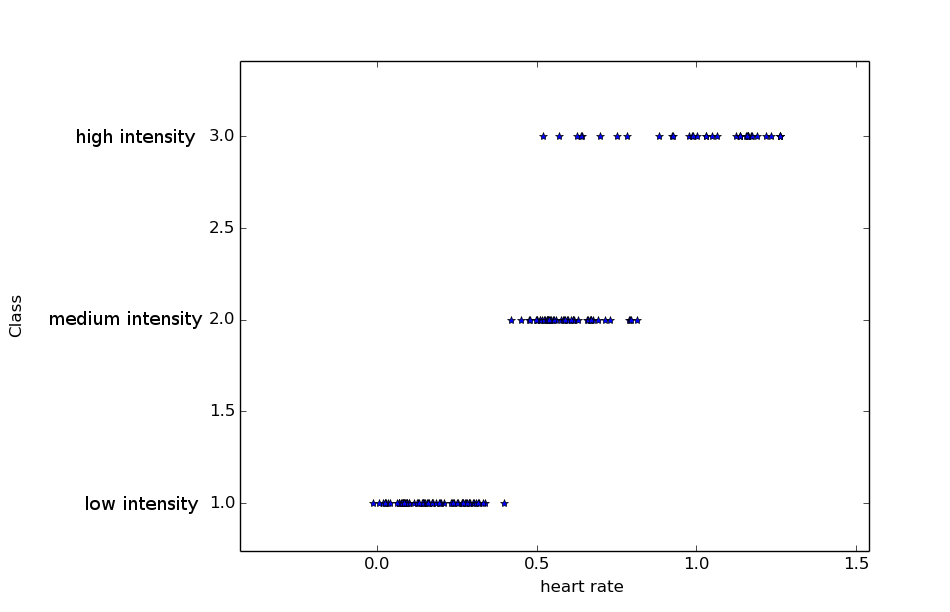
\includegraphics[width=130mm]{pictures/plot_multiclass_data.png}
  \caption{Plotting of three classes for feature heart rate \label{multi-class-data}}
\end{figure}

\begin{figure}[ht!]
  \centering
  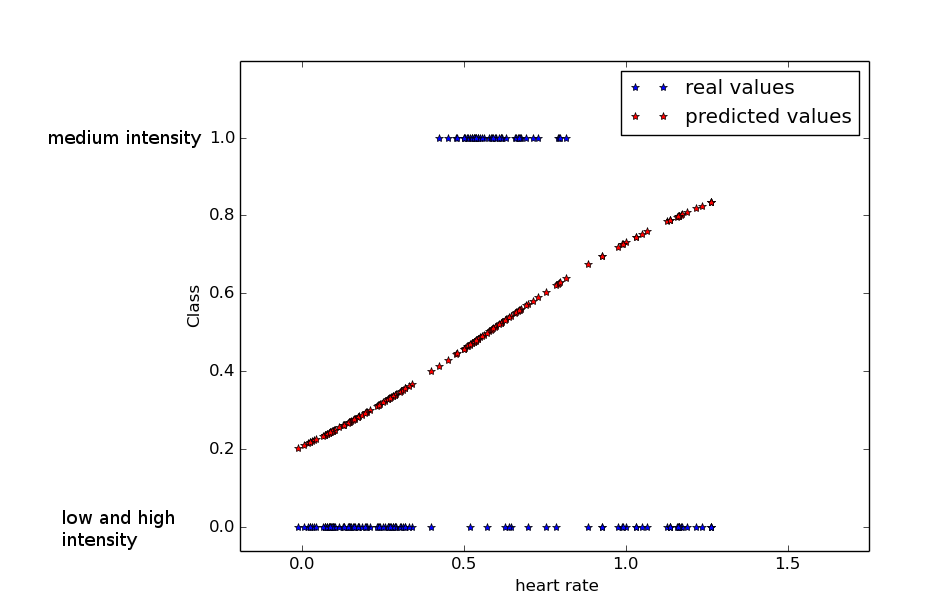
\includegraphics[width=130mm]{pictures/one-vs-all_classification.png}
  \caption{Trying to fit sigmoid function for one-vs-all approach \label{one-vs-all}}
\end{figure}

We also tested using regularization. This is a method which tries to reduce overfitting by penalizing high parameter values in the model. However, this did not improve our results.

In our implementation there are two main parameters that can be optimized. The first one is the number of iterations for the gradient ascent. We tested values between 100 and 9000. From about 1000 iterations on, the result is only improving slightly if more iterations are added. We settled for 1500 iterations. The second parameter is alpha, which determines how big the steps in each iteration of the gradient ascent are. There we tested values between 0.001 and 10. 0.1 was the best value of the results. Those tests were done on a random two-way split on one subject. Ideally would be a three-way split (training, parameter optimization, testing). However, as it was only done on one subject, all the testing data from the other subjects have not been seen before doing the actual testing. Therefore the testing results are still valid.


\subsection{Locally Weighted Linear Regression}

The main idea in locally weighted linear regression is to build a new local model of the function, whenever a sample should be classified and then use it to predict the output value. Therefore instead of using a model-based method such as linear and logistic regression and building a parameterized model for prediction, it acts as a memory-based method and uses the whole training dataset, each time a prediction for a new datapoint has to be made. Thus the only difference between this type of regression and a simple regression model is using a weight matrix W (equation (\ref{eq:weight_matrix})) as one of the model parameters. Equation (\ref{eq:lwr_wght_theta}) is a model of the parameters.

\begin{equation}
\label{eq:weight_matrix}
W = \begin{bmatrix}
w_{(1,1)}	& 0	& \dots	 & 0      \\
0	& w_{(2,2)} 	& \dots  & 0 	  \\
\vdots	& 0 	& \ddots & \vdots \\
0 	& \dots & 0	 & w_{(n,n)}
\end{bmatrix}
\end{equation}

\begin{equation}
\label{eq:lwr_wght_theta}
 \Theta = (X^TWX)^{-1}X^TWy
\end{equation}

To get the prediction, we need to multiply $\Theta$ with our inputs x, which is shown in equation (\ref{eq:lwr_final}).


\begin{equation}
\label{eq:lwr_final}
 h_\Theta(x) = \Theta^Tx
\end{equation}


The reason that this algorithm re-builds the local model for every input datapoint, is to assign new weights to the training data, so that nearby points get more weights. This however, makes the locally weighted regression algorithm computationally much more expensive comparing to other approaches discussed in this paper.

\begin{figure}[ht!]
  \centering
  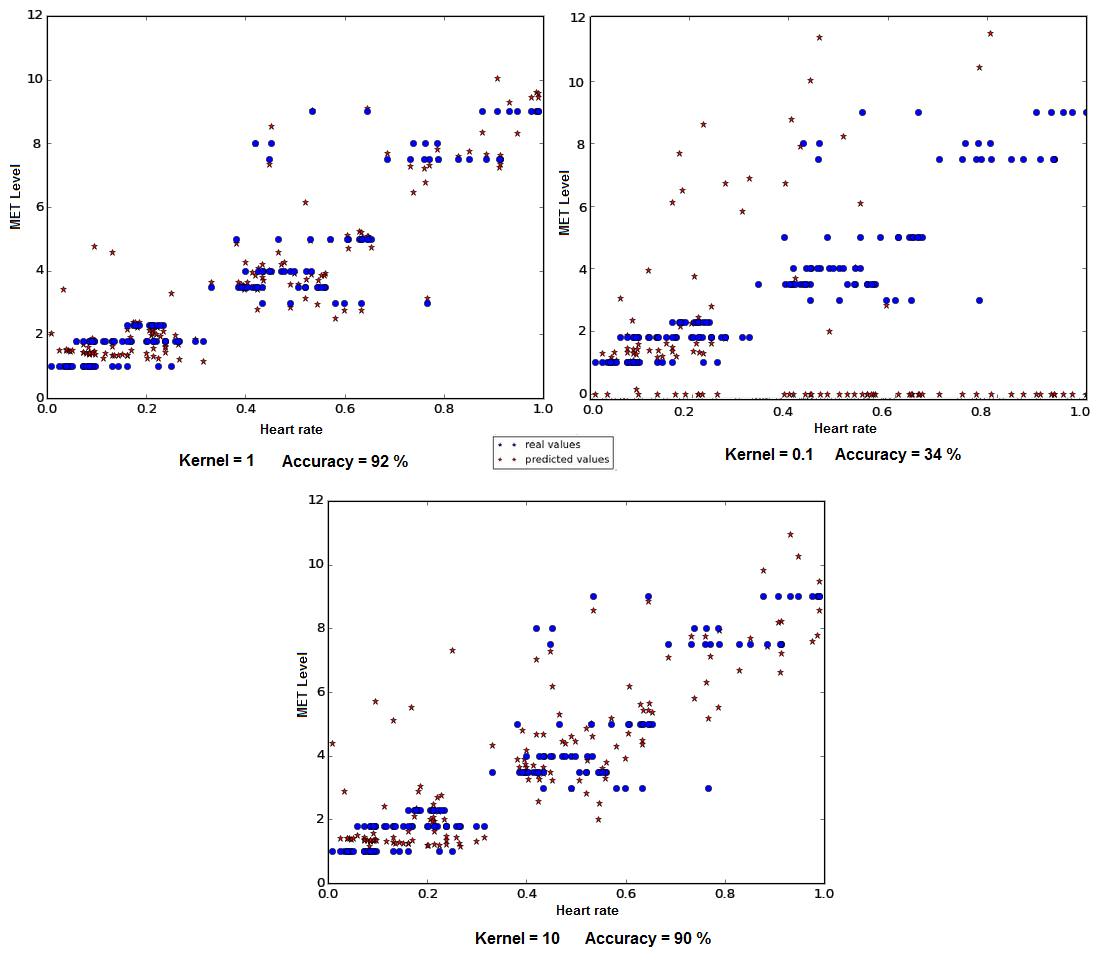
\includegraphics[width=160mm]{pictures/lwr_3_kernel_constants5.png}
  \caption{Result of different constants for exponential kernel
  \label{lwr_3_kernel}}
\end{figure}

In addition, by kernel smoothing, the algorithm smooths out the new point of interest using nearby datapoints. We used the exponential kernel function, which uses $\sigma$ as the smoothing parameter. The function is calculating the weights that should be assigned to x, the datapoint that we want to predict. These datapoints are denoted by $x^{(i)}$. 

\begin{eqnarray}
w_{(i,i)} &=& exp(-\frac{||x^{(i)}-x||}{2\sigma^2})
\end{eqnarray}



It is significant to note that in order to avoid overfitting and underfitting, one must pick good kernel parameters. Figure \ref{lwr_3_kernel} shows the results of executing the algorithm on the dataset, each time with a different value for the kernel constant. A large value takes a lot of points into account, even the ones that are so far away, and consequently generalizes too much.

On the other hand, for a small value, all points are neglected, except the ones that are very close to the test point, and as a result the model overfits the data. In our case, the algorithm fails for some of the test datapoints and cannot find any result.

\subsection{AdaBoost}

AdaBoost uses Boosting to improve the classification results. Boosting means that the same classifier (base-level or "weak" classifier) is used multiple times. In each iteration the training data samples get different weights, thereby making the classifier to focus on a subset of the training data. This results in a set of "weak" classifiers. For a new sample we run all of the "weak" classifiers we trained and do a majority vote. The majority vote is weighted based on the classifier's accuracy on training data.

The Algorithm is based on the concept of "weak" classifiers: It should be better than random guessing (e.g. binary classification, accuracy \textgreater 50\%) but not too good. Otherwise it is in danger of overfitting.

As algorithm for these "weak" classifiers we can use any algorithm that supports weighting of training samples, for example:
\begin{itemize}
\item decision tree
\item kNN
\end{itemize}

We decided to use decision trees, as this is also the base classifier in the AdaBoost implementation of scikit learn \cite{scikit_adaboost_doc}.

We started by using full depth decision trees, as we thought: Using a better performing classifier as base classifier can not be bad. However, this resulted in accuracies around 0.7. After a lot of investigation we realized that it really makes a difference if you use a "strong" or a "weak" classifier. So we used decision trees with maximum depth 2 and this improved our scores to over 0.9.

As parameter for the number of iterations / the number of base classifiers we chose 50. This is the default value used in the Scikit implementation of AdaBoost. It offers a good trade-off between accuracy and performance.


\section{Results and Discussion}

Finally we evaluated all of our classifiers as well as the corresponding scikit learn implementations. We did three different kinds of cross validation
\begin{itemize}
\item Leave-on-subject-out Cross-Validation \newline
We run the classifier as many times as we have subjects. Each time using one subject as testing data and the rest as training data. This is the most meaningful score in practice. In a real world application you would train your model on all the data you have and then it would have to deal with the data from a user it has not seen before.
\item 10-fold Cross-Validation over all the data\newline
This is simple 10-fold Cross-Validation over all subject.
\item 10-fold Cross-Validation on each subject\newline
In this testing case we look at all subjects independently, do a 10-fold Cross-Validation on each one of them and then take the mean of all of the results.
\end{itemize}

As scoring measure we took accuracy. Since our classes are pretty balanced, accuracy provides a good measure.

\begin{table}
  \begin{tabular}{ l | c | c | c }
     & LOSO CV & 10-fold CV & 10-fold CV OES  \\ \hline
    Scikit AdaBoost (SAMME) & 0.86 & 0.85 & 0.92 \\ \hline
    Custom AdaBoost (M1) & 0.93 & 0.98 & 0.99 \\ \hline
    Scikit Decision Tree & 0.89 & 0.97 & 0.96 \\ \hline
    Scikit Logistic Regression & 0.91 & 0.93 & 0.97 \\ \hline
    Custom Logistic Regression & 0.86 & 0.88 & 0.96 \\ \hline
    Scikit Linear Regression & 0.92 & 0.91 & 0.92 \\ \hline
    Custom Linear Regression & 0.91 & 0.91 & 0.92 \\ \hline
    Custom Locally Weighted Reg & 0.89 & 0.88 & 0.89 \\ \hline
  \end{tabular}
  \caption{Classificiation Results; the scores are accuracies (column names: LOSO CV: Leave-one-subject-out Cross-Validation; 10-fold CV: 10-fold Cross-Validation; 10-fold CV OES: 10-fold Cross-Validation on each subject \label{results-table}}
\end{table}

In the following we will only talk about the Leave-on-subject-out Cross-Validation score, as this one is most significant for real life applications.
\newline We achieved the best score with our Custom AdaBoost (M1) implementation. It is quite interesting that it outperformed the Scikit AdaBoost (SAMME) implementation. SAMME is supposed to be a bit more advanced than M1 and the Scikit implementation was certainly a lot more optimised than our implementation. The main reason for our better performance is this: We used decision trees with maximum depth 2 whereas the Scikit implementation uses decision trees with maximum depth 1. However, for other problems maximum depth 1 might work better and probably that's the reason why they chose this value.

Overall the scores of all the algorithms do not differ a lot. We did not check if these differences are significant, but one has to doubt it.

\begin{table}
  \begin{tabular}{ l | c | c }
     & performance train & performance perdict \\ \hline
    Scikit AdaBoost (SAMME) & 300 & 19 \\ \hline
    Custom AdaBoost (M1) & 700 & 2230 \\ \hline
    Scikit Decision Tree & 56 & 0.4 \\ \hline
    Scikit Logistic Regression & 90 & 0.4 \\ \hline
    Custom Logistic Regression & 1950 & 11 \\ \hline
    Scikit Linear Regression & 2 & 0.07 \\ \hline
    Custom Linear Regression & 1940 & 3 \\ \hline
    Custom Locally Weighted Reg & no previous training & 15min 25s \\ \hline
  \end{tabular}
  \caption{Performance Results in ms \label{results-table-performance}}
\end{table}

Regarding the performance of the algorithms, the time it takes to predict is the more interesting one for real life applications. Here we see that the Scikit Linear Regression is  by far the fastest. Considering the simplicity of the mathematical model behind it, that makes sense. The predict performance of the Custom AdaBoost (M1) is slow, because we did not optimize it with vector operations, but used a simple for loop to do predictions for a range of samples. If we measure the time for prediction for only one sample, our implementation is even faster than the Scikit AdaBoost implementation.

The long training time of our logistic and linear regression implementation is due to the use of gradient ascent with many iterations to estimate the parameters. The Scikit Implementations probably use numerical solutions and are a lot more optimized. That explains their better performance.

Wrapping everything up, we can see that estimating the intensity level of an activity from just a few sensors worn at the body, is easily possible with standard Machine Learning Algorithms and with high accuracy.
For a real life application we would suggest using the Scikit Linear Regression implementation. It offers almost as good accuracy as the Custom AdaBoost implementation, but has a lot better performance on training and prediction. Moreover, it needs less memory, as we only have to save the parameters for the linear function. AdaBoost instead has to save the entire set of base classifiers.


%END OF DOCUMENT / BEGIN OF APPENDIX
\newpage
\pagestyle{plain}
\pagenumbering{Roman}
\appendix

%Code Listings
\phantomsection\addcontentsline{toc}{section}{Code Listings}\section*{Code Listings}

Find the source code in the ZIP file we also provided.


%References
%\newpage %adds a page break between Code Listings and References
\phantomsection\addcontentsline{toc}{section}{References}

\begin{thebibliography}{99}
%Be aware of the correct order!

\bibitem{Attila_2012}
  Attila Reiss, Didier Stricker: \emph{Creating and Benchmarking a New Dataset for Physical Activity Monitoring}. In: 5th Workshop on Affect and Behaviour Related Assistance (ABRA), June 6-8, 2012, Crete, Greece, 2012.
   
\bibitem{Attila_2013}
  Attila Reiss, Didier Stricker:
  \emph{Aerobic activity monitoring: towards a long-term approach}, 2013.

\bibitem{Attila}
  Barbara E. Ainsworth, William L. Haskell, Melicia C. Whitt, Melinda L. Irwin, Ann M. Swartz, Scott J. Strath, William L. O'Brien, David R. Bassett, Jr., Kathryn H. Schmitz, Patricia 0. Emplaincourt, David R. Jacobs, Jr. and Arthur S. Leon:
  \emph{Compendium of Physical Activities: an
update of activity codes and
MET intensities},
  2012.
  

    
\bibitem{scikit_adaboost_doc}
	http://scikit-learn.org/stable/modules/generated/sklearn.ensemble.AdaBoostClassifier.html
  
  
  
\bibitem{learning_rate}
Open classeroom, Machine Learning Lecture 13 of 30, \emph{Linear Regression II: Learning Rate} , 12-02-2015
\href{http://openclassroom.stanford.edu/MainFolder/VideoPage.php?course=MachineLearning&video=03.2-LinearRegressionII-LearningRate}{[Link]}  
\bibitem{learning_rate}
Marcel Caraciolo, \emph{Machine Learning with Python - Linear Regression} , 12-02-2015
\href{http://aimotion.blogspot.de/2011/10/machine-learning-with-python-linear.html}{[Link]}


\bibitem{ACSM}
W. L. Haskell, I.-M. Lee, R. R. Pate, K. E. Powell, S. N. Blair, B. a. Franklin, C. a. Macera, G. W. Heath, P. D. Thompson, and A. Bauman. Physical activity and public health: updated recommendation for adults from the American College of Sports Medicine and the American Heart Association. \emph{Medicine and science in sports and exercise,} 39(8):1423–1434, Aug. 2007.

\bibitem{PAMAP_2}
http://www.pamap.org/demo.html

\bibitem{met_paper}
B. E. Ainsworth, W. L. Haskell, M. C. Whitt, M. L.
Irwin, a. M. Swartz, S. J. Strath, W. L. O'Brien, D. R.
Bassett, K. H. Schmitz, P. O. Emplaincourt, D. R.
Jacobs, and a. S. Leon. Compendium of physical
activities: an update of activity codes and MET
intensities. \emph{Medicine and science in sports and
exercise}, 32(9):498-504, Sept. 2000.

\end{thebibliography}

%List of Figures
%\newpage %adds a page break between References and List of Figures
\phantomsection\addcontentsline{toc}{section}{List of Figures}\listoffigures

%List of Tables
%\newpage %adds a page break between List of Figures and List of Tables
\phantomsection\addcontentsline{toc}{section}{List of Tables}\listoftables

%List of Listings
%\newpage %adds a page break between List of Tables and List of Listings
%\phantomsection\addcontentsline{toc}{section}{List of Listings}\lstlistoflistings
\end{document} 